%% LICENCE: CC-BY-NC-SA
%% Copyright: Jesús Espino
%% Based on Git Internals chapter of ProGit book (http://git-scm.com/book)
\documentclass[10pt]{beamer}

\usepackage[utf8]{inputenc}
\usepackage[spanish]{babel}
\usepackage{graphicx}

\mode<presentation>
\usetheme{Madrid}
%\usecolortheme[RGB={111,73,135}]{structure}
\usecolortheme[RGB={128,0,0}]{structure}
%\usecolortheme[RGB={0,96,0}]{structure}
%\usecolortheme[RGB={200,0,200}]{structure}
%\usecolortheme[RGB={0,128,0}]{structure}
%\usecolortheme[RGB={0,0,128}]{structure}
\usefonttheme{serif}
\useinnertheme{rectangles}
\useoutertheme{split}

\setbeamercovered{transparent}

\title{Git Internals}
\author{Jesús Espino García}
\date{19 de Abril de 2013}
\subject{Git Internals}

\institute[Kaleidos]{jesus.espino@kaleidos.net\\@jespinog\\
\includegraphics[height=1.5cm]{kaleidos.png}}

\setcounter{tocdepth}{2}

\AtBeginSubsection[]
{
  \begin{frame}[containsverbatim]<beamer>{Indice}
    \tableofcontents[sectionstyle=show/shaded,subsectionstyle=show/shaded/hide]
  \end{frame}
}

\begin{document}

  \frame{\maketitle}

  \section*{Introducción}

  \begin{frame}[containsverbatim]
    \frametitle{¿Por qué?}
    \begin{itemize}
      \item La interfaz de git es de bajo nivel.
      \item Conocer git bien da mucho poder.
      \item El poder está ahí aunque no lo conozcamos.
      \item Un gran poder conlleva una gran responsabilidad.
    \end{itemize}
  \end{frame}

  \begin{frame}[containsverbatim]
    \frametitle{Conceptos básicos}
    \begin{itemize}
        \item Procelain (Porcelana).
        \item Plumbing (Cañerias).
        \item Objetos
        \item Referencias
        \item Head
        \item Working copy
    \end{itemize}
  \end{frame}

  \begin{frame}[containsverbatim]
    \frametitle{Contenido de .git}
    \begin{itemize}
        \item Ficheros.
        \begin{itemize}
            \item HEAD
            \item index
            \item config
        \end{itemize}
        \item Directorios.
        \begin{itemize}
            \item objects
            \item refs
            \item hooks
            \item info
        \end{itemize}
    \end{itemize}
  \end{frame}

  \section*{Objetos}

  \begin{frame}[containsverbatim]
    \frametitle{Objetos}
    \begin{itemize}
        \item Bloque de datos almacenado en git
        \item Referenciado por el sha1 de su contenido
        \item Almacenados en el directorio \verb$.git/objects/$ (o en packs).
        \item Hay 4 tipos de objetos en git (blob, tree, commit, tag).
    \end{itemize}
  \end{frame}

  \begin{frame}[containsverbatim]
    \frametitle{blobs}
    \begin{itemize}
        \item Será el nodo hoja de nuestros arboles.
        \item Será equivalente (normalmente) a nuestros ficheros.
    \end{itemize}
  \end{frame}

  \begin{frame}[containsverbatim]
    \frametitle{Ejemplo de almacenar blob}
    \begin{itemize}
        \item \verb$git init repo; cd repo$
        \item \verb$echo 'version 1' | git hash-object -w --stdin$
        \item \verb$find .git/objects -type f$
        \item \verb$git cat-file -p 83baae61804e65cc73a7201a7252750c76066a30$
        \item \verb$echo 'version 2' | git hash-object -w --stdin$
        \item \verb$find .git/objects -type f$
        \item \verb$git cat-file -p 1f7a7a472abf3dd9643fd615f6da379c4acb3e3a$
    \end{itemize}
  \end{frame}

  \begin{frame}[containsverbatim]
    \frametitle{trees}
    \begin{itemize}
        \item Es un directorio de referencias a blob y otros trees.
        \item Almacena referencias (sha1 de objetos) y metadatos.
    \end{itemize}
  \end{frame}

  \begin{frame}[containsverbatim]
    \frametitle{diagrama de ejemplo de trees}
    \begin{center}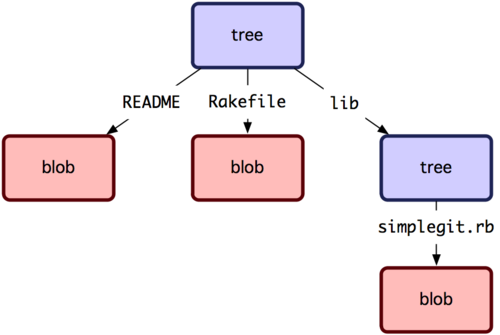
\includegraphics{trees.png}\end{center}
  \end{frame}

  \begin{frame}[containsverbatim]
    \frametitle{Ejemplo de almacenar tree}
    \begin{itemize}
        \item \verb$git init repo; cd repo$
        \item \verb$git update-index --add --cacheinfo 100644 \$ \verb$83baae61804e65cc73a7201a7252750c76066a30 test.txt$
        \item \verb$git write-tree$
        \item \verb$find .git/objects -type f$
        \item \verb$git cat-file -p d8329fc1cc938780ffdd9f94e0d364e0ea74f579$
    \end{itemize}
  \end{frame}

  \begin{frame}[containsverbatim]
    \frametitle{commits}
    \begin{itemize}
        \item Almacena una referencia a un tree.
        \item Almacena una referencia a su commit padre.
        \item Almacena metadatos del commit (autor, fecha, mensaje...)
    \end{itemize}
  \end{frame}

  \begin{frame}[containsverbatim]
    \frametitle{diagrama de ejemplo de commits}
    \begin{center}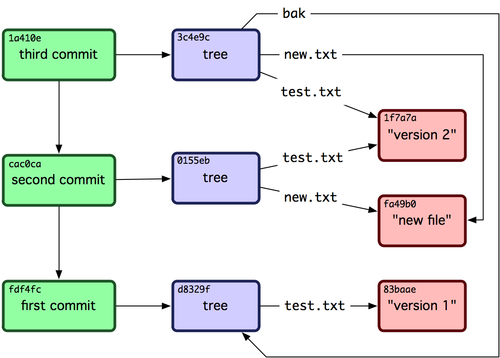
\includegraphics{commits.png}\end{center}
  \end{frame}

  \begin{frame}[containsverbatim]
    \frametitle{Ejemplo de commit}
    \begin{itemize}
        \item \verb$git init repo; cd repo$
        \item \verb$echo "Version 1" > fichero.txt; git add fichero.txt$
        \item \verb$git commit -m "Version 1"$
        \item \verb$find .git/objects -type f$
        \item \verb$git cat-file -p HEAD$
        \item \verb$git cat-file -p b7c0dba424af1e98a3570f8125476126129e5c32$
        \item \verb$git cat-file -p fb8247c7b27ae4cad9e7e3e66ba95126658ea7c2$
    \end{itemize}
  \end{frame}

  \begin{frame}[containsverbatim]
    \frametitle{tags}
    \begin{itemize}
        \item Almacena una referencia a un commit.
        \item Almacena metadatos del commit (autor, fecha, nombre...)
    \end{itemize}
  \end{frame}

  \begin{frame}[containsverbatim]
    \frametitle{Objects storage}
    \begin{itemize}
        \item Se añade una cabecera con el tipo de objeto y la longitud del mismo.
        \item Se concatena con los datos que se van a almacenar
        \item Se calcula su sha1 que se utilizara como nombre del objeto.
        \item Se comprime con zlib.
        \item Se almacena en \verb$.git/objects/XX/XXXXXX$\dots{}
    \end{itemize}
  \end{frame}

  \begin{frame}[containsverbatim]
    \frametitle{Ejemplo de lectura directa}
    \begin{itemize}
        \item \verb$git init repo; cd repo$
        \item \verb$echo "Version 1" > fichero.txt; git add fichero.txt$
        \item \verb$git commit -m "Version 1"$
        \item \verb$find .git/objects -type f$
        \item \verb$git cat-file -p HEAD$
        \item \verb$git cat-file -p b7c0dba424af1e98a3570f8125476126129e5c32$
        \item \verb$git cat-file -p fb8247c7b27ae4cad9e7e3e66ba95126658ea7c2$
        \item \verb$cat .git/objects/fb/8247c7b27ae4cad9e7e3e66ba95126658ea7c2 \$ \verb$| zlib-flate -uncompress$
    \end{itemize}
  \end{frame}

  \section*{Packfiles}

  \begin{frame}[containsverbatim]
    \frametitle{Packfiles}
    \begin{itemize}
        \item Paquetes de objetos.
        \item Periodicamente git empaqueta los objetos en packs (gc).
        \item Se almacenan en \verb$.git/objects/pack/$.
        \item Hay un listado de packs en \verb$.git/objects/info/packs$.
        \item Cada pack tiene su indice en \verb$.git/objects/pack/$.
    \end{itemize}
  \end{frame}

  \section*{Referencias}

  \begin{frame}[containsverbatim]
    \frametitle{Referencias}
    \begin{itemize}
        \item Están en \verb$.git/refs$ principalmente.
        \item Son punteros a objetos.
        \item Contienen el id del objeto al que apuntan.
    \end{itemize}
  \end{frame}

  \begin{frame}[containsverbatim]
    \frametitle{branchs}
    \begin{itemize}
        \item Están en \verb$.git/refs/heads$
    \end{itemize}
  \end{frame}

  \begin{frame}[containsverbatim]
    \frametitle{HEAD}
    \begin{itemize}
        \item Esta en \verb$.git/HEAD$
        \item Es una referencia simbolica que apunta a la referencia de la rama actual.
    \end{itemize}
  \end{frame}

  \begin{frame}[containsverbatim]
    \frametitle{tags}
    \begin{itemize}
        \item Están en \verb$.git/refs/tags$
        \item Son referencias a commits o a objetos tag.
        \item Los tags simples son una referencia directa a un commit.
        \item Los tags con anotaciones son referencias a un objeto tag que apunta a un commit.
    \end{itemize}
  \end{frame}

  \begin{frame}[containsverbatim]
    \frametitle{remotes}
    \begin{itemize}
        \item Están en \verb$.git/refs/remotes$
        \item Contiene las referencias de mis remotes.
        \item Se actualizan cuando hago push o fetch.
    \end{itemize}
  \end{frame}

  \begin{frame}[containsverbatim]
    \frametitle{Refspects}
    \begin{itemize}
        \item Forma de definir la relación entre las referencias de diferentes origines
        \item Tienen el formato \verb$[+]<src>:<dst>$
        \item Opcionalmente se pone un \verb$+$ para actualizar la referencia cuando no hay fast-forward.
        \item Las referencias pueden tener \verb$*$ para definir "todo lo que haya en un directorio"
        \item No se permite el uso de \verb$*$ para selecciones parciales de referencias.
        \item Ejemplo: \verb$+refs/heads/*:refs/remotes/origin/*$
    \end{itemize}
  \end{frame}

  \begin{frame}[containsverbatim]
    \frametitle{Pulling with refspects}
    \begin{itemize}
        \item Ejemplo: \verb$git fetch origin master:refs/remotes/origin/mymaster$
        \item Descarga la referencia master del origin a \verb$refs/remotes/origin/mymaster$ en local
    \end{itemize}
  \end{frame}

  \begin{frame}[containsverbatim]
    \frametitle{Pushing with refspects}
    \begin{itemize}
        \item Ejemplo: \verb$git push origin master:refs/heads/qa/master$
        \item Envia la referencia master local al \verb$refs/heads/qa/master$ en origin
    \end{itemize}
  \end{frame}

  \begin{frame}[containsverbatim]
    \frametitle{Borrando referencias}
    \begin{itemize}
        \item Ejemplo: \verb$git push origin :topic$
        \item Borra la referencia topic en origin
    \end{itemize}
  \end{frame}

  \section*{Hablemos de algunos comandos}

  \begin{frame}[containsverbatim]
    \frametitle{init}
    Crea un .git con datos básicos.
    \begin{itemize}
      \item Un fichero config por defecto.
      \item Los directorios refs, objects e info.
      \item Un \verb+HEAD+ apuntando a la referencia master.
      \item Y poco más
    \end{itemize}
  \end{frame}

  \begin{frame}[containsverbatim]
    \frametitle{add}
    \begin{itemize}
      \item Añade el fichero a la base de datos de Objetos.
      \item Añade el fichero al index.
    \end{itemize}
  \end{frame}

  \begin{frame}[containsverbatim]
    \frametitle{commit}
    \begin{itemize}
      \item Añade el tree apuntando al arbol de ficheros al que apunte el index a la base de datos de objetos.
      \item Añade el commit apunte al tree recien añadido a la base de datos de objetos.
      \item Modifica el \verb+HEAD+.
      \item Modifica la referencia de la rama actual.
    \end{itemize}
  \end{frame}

  \begin{frame}[containsverbatim]
    \frametitle{checkout}
    \begin{itemize}
      \item Compara el tree del commit actual y el tree del commit destino.
      \item Extrae los objetos diferentes entre ambos a la working copy.
      \item Si existen ficheros modificados intenta hacer el merge y conservar las modificaciones.
      \item Modifica el \verb+HEAD+.
    \end{itemize}
  \end{frame}

  \begin{frame}[containsverbatim]
    \frametitle{reset}
    \begin{itemize}
      \item Modifica la referencia a la que apunte \verb+HEAD+ y la apunta al commit que le digas.
      \item Depende del tipo de reset modifica el index para ajustarlo al nuevo commit.
      \item Depende del tipo de reset modifica la working copy para ajustarlo al nuevo commit.
    \end{itemize}
  \end{frame}

  \begin{frame}[containsverbatim]
    \frametitle{rebase}
    \begin{itemize}
      \item Se posiciona en la rama destino.
      \item Añade los commits de la rama origen uno a uno en la rama destino.
      \item Si hay comflicto los resuelve (automatica o manualmente) modificando el commit.
      \item Actualiza la referencia de ambas ramas para apuntar al último commit.
    \end{itemize}
  \end{frame}

  \begin{frame}[containsverbatim]
    \frametitle{merge}
    \begin{itemize}
      \item Pregunta por el origen comun de las ramas a mergear.
      \item Calcula las diferencias que genera cada rama.
      \item Intenta mezclar las diferencias en un nuevo commit.
      \item Si hay comflicto los resuelve (automatica o manualmente).
      \item Genera un objeto commit (con varios parents) con las diferencias de ambos aplicadas.
      \item Actualiza la referncia de la rama destino al nuevo commit.
    \end{itemize}
  \end{frame}

  \section*{Para terminar}

  \begin{frame}[containsverbatim]
    \frametitle{¿De qué no hemos hablado?}
    \begin{itemize}
        \item Más comandos de porcelana.
        \item Comandos de plumbing.
        \item Protocolos de transferencia.
        \item Mantenimiento y recuperación de datos.
        \item Stash
        \item fsck
        \item Other files internal format (index, packs, pack-idx\dots{})
    \end{itemize}
  \end{frame}

  \begin{frame}[containsverbatim]
    \frametitle{Referencias}
    \begin{itemize}
      \item \small{http://git-scm.com/ - Web oficial de git.}
      \item \small{http://git-scm.com/book - ProGit (El libro de Git).}
      \item \small{Documentation/technical - Technical doc in the git respoitory. }
      \item \small{http://gitguys.com/ - Página sobre git.}
      \item \small{http://github.com/ - Servicio de git por excelencia.}
      \item \small{http://bitbucket.org/ - Servicio de git de repositorios privados gratis.}
    \end{itemize}
  \end{frame}

  \begin{frame}[containsverbatim]
    \frametitle{Dudas}
    \dots
  \end{frame}

\end{document}
